\chapter{Forces, espace des phases et lois de conservation}

\lectureoverview{Une loi du mouvement doit faire plus que relier des grandeurs physiques familières. Elle doit spécifier l’état d’un système, faire évoluer cet état d’un instant au suivant et révéler quelles distinctions et quelles grandeurs subsistent au cours du mouvement. Nous aborderons la mécanique newtonienne en examinant d’abord une loi des forces plausible mais erronée, puis en élargissant l’état, de la position à l’espace des phases, et enfin en dérivant les lois de conservation de la quantité de mouvement et de l’énergie.}

\section{Une loi erronée, mais instructive}

Le mouvement quotidien est dominé par le frottement. Poussez un objet lourd sur un sol : il se déplace ; cessez de pousser et il s’arrête bientôt. En général, une poussée plus forte produit une vitesse plus grande, tandis qu’un objet plus lourd exige une poussée plus forte. Dans un tel monde, il est naturel de supposer que la force produit directement la vitesse. C’était l’intuition fondamentale qui sous-tendait la description aristotélicienne du mouvement.

Le patinage sur glace apporte l’expérience qui manque. Un patineur a besoin d’une force pour démarrer, s’arrêter ou changer de direction, mais pas pour continuer à glisser une fois en mouvement. Si Aristote avait travaillé sur une glace presque sans frottement plutôt que sur un sol ordinaire, le défaut de l’intuition force--vitesse aurait été beaucoup plus difficile à repérer.

Pour mettre en évidence ce qui cloche dans cette intuition, donnons-lui une formulation moderne précise. Écrivons l’équation délibérément incorrecte

\begin{equation}
  \mathbf F=m\mathbf v.
  \label{eq:aristotle-vector-law}
\end{equation}

Ce n’est pas la loi de Newton et il ne faut pas la mémoriser comme une loi physique. Elle est utile à titre diagnostique : une fois qu’une règle verbale est devenue une équation, nous pouvons demander si elle prédit le mouvement et si elle conserve suffisamment d’information pour reconstruire le passé. La brève discussion en classe du mot grec désignant la force renvoie à \emph{dynamis}, dont la racine se retrouve aussi dans des mots comme dynamo et dynamique ; mais la terminologie compte moins que la mise à l’épreuve de la loi elle-même.

\begin{figure}[htbp]\centering
  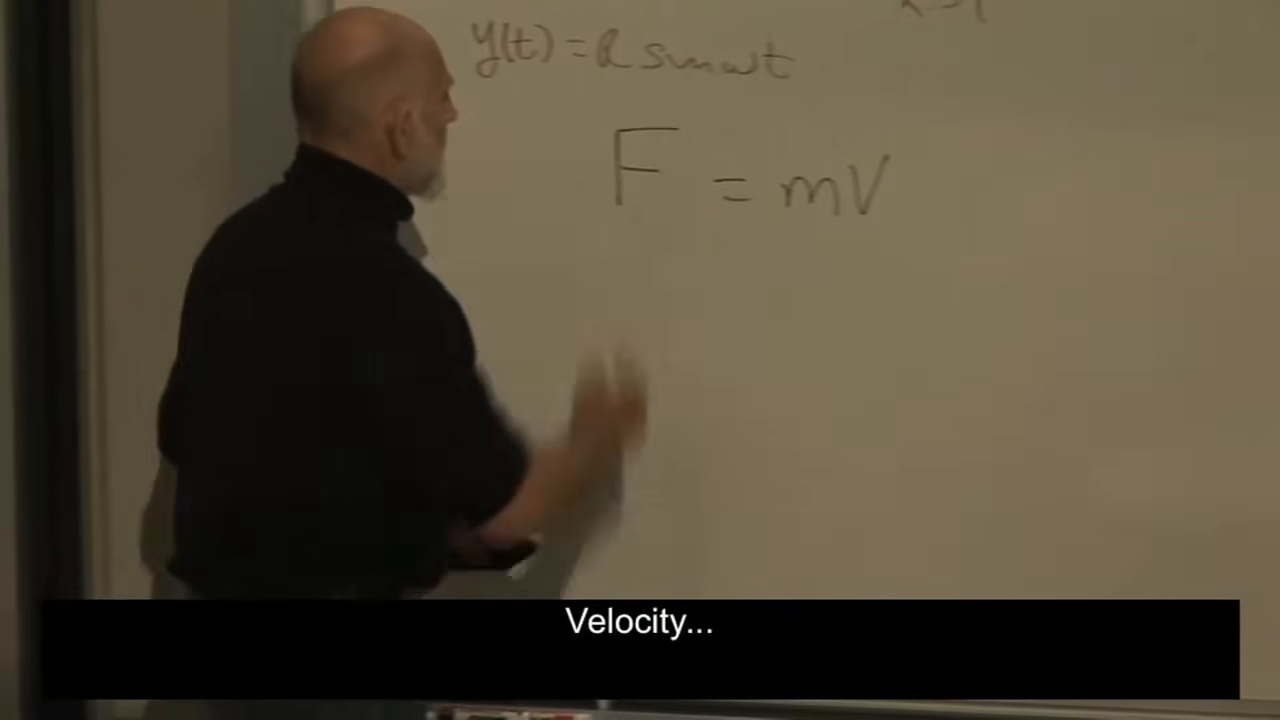
\includegraphics[width=0.82\textwidth]{lecture_02_figure_02.png}\caption{La loi force--vitesse, volontairement erronée, utilisée pour tester la prédictibilité et la réversibilité.}\lectureframe{00:04:51}\end{figure}

Restreignons le mouvement à une seule coordonnée spatiale. Puisque \(v=\dot x\), la loi s’écrit

\begin{equation}
  F(t)=m\dot x(t).
  \label{eq:aristotle-1d}
\end{equation}

Divisons maintenant le temps en courts intervalles de durée \(\delta\). Sur un intervalle,

\begin{equation}
  \dot x(t)\simeq
  \frac{x(t+\delta)-x(t)}{\delta}.
  \label{eq:first-difference}
\end{equation}

En substituant dans l’équation~\eqref{eq:aristotle-1d}, on obtient

\begin{equation}
  x(t+\delta)
  =x(t)+\frac{\delta}{m}F(t).
  \label{eq:aristotle-update}
\end{equation}

On a là la forme d’une véritable règle de mise à jour. Si l’on connaît la position actuelle et la force, on peut déterminer la position à l’instant stroboscopique suivant. Toutefois, lorsque la force s’annule, la règle d’Aristote donne \(\dot x=0\) : l’objet doit rester au repos. Le mouvement sans force d’entretien est exclu d’emblée.

\begin{figure}[htbp]\centering
  \includegraphics[width=0.84\textwidth]{lecture_02_figure_07.png}\caption{La mise à jour discrète d’Aristote avec une force de rappel. À chaque étape, le déplacement est multiplié par un facteur légèrement inférieur à un.}\lectureframe{00:10:15}\end{figure}

\subsection{Un ressort dans la mécanique d’Aristote}

Considérons une particule attachée à un ressort, dont la position d’équilibre est \(x=0\). Un déplacement produit la force de rappel

\begin{equation}
  F(x)=-kx,
  \qquad k>0.
  \label{eq:hooke-law}
\end{equation}

En introduisant cette force dans l’équation~\eqref{eq:aristotle-update}, on obtient

\begin{equation}
  x(t+\delta)
  =\left(1-\frac{k\delta}{m}\right)x(t).
  \label{eq:aristotle-spring-update}
\end{equation}

Pour \(\delta\) suffisamment petit, le facteur entre parenthèses est légèrement inférieur à un. Chaque mise à jour réduit donc le déplacement dans la même proportion :

\begin{equation}
  x_n=\left(1-\frac{k\delta}{m}\right)^n x_0.
  \label{eq:aristotle-geometric-decay}
\end{equation}

L’équation continue et sa solution sont

\begin{align}
  m\dot x&=-kx,
  \label{eq:aristotle-spring-continuous}\\
  x(t)&=x(0)e^{-kt/m}.
  \label{eq:aristotle-spring-solution}
\end{align}

Le ressort n’oscille pas. Quelle que soit la position initiale dont on la libère, la particule s’approche de l’origine de façon exponentielle, en ralentissant à mesure qu’elle s’en rapproche.

\begin{figure}[htbp]\centering
  \includegraphics[width=0.84\textwidth]{lecture_02_figure_08.png}\caption{La solution exponentielle de l’équation aristotélicienne du ressort. Le déplacement décroît au lieu d’osciller.}\lectureframe{00:12:02}\end{figure}

L’avenir est facile à prédire : tout déplacement initial tend vers la même configuration de repos. Pour le passé, c’est une autre affaire. Supposons que la particule soit observée très près de l’origine, avec une précision finie seulement. Elle aurait pu partir de n’importe laquelle de nombreuses positions distinctes, car leurs traces, devenues exponentiellement petites, finissent toutes par se trouver dans la même marge d’incertitude de mesure. Avec une précision mathématique parfaite, l’équation~\eqref{eq:aristotle-spring-solution} peut être résolue à rebours, mais les distinctions pratiques entre les histoires possibles s’effacent peu à peu. Du point de vue de la dynamique fondamentale réversible, cette loi est donc suspecte.

Cela ne signifie pas qu’Aristote était irrationnel. Le mouvement dominé par le frottement qu’il décrivait est effectivement dissipatif. Son erreur a été d’ériger ce comportement effectif en loi fondamentale. Le frottement est lui-même une force qui découle d’interactions microscopiques complexes. Lorsqu’une main pousse un objet à une vitesse à peu près constante, la force appliquée compense le frottement ; elle ne crée pas la vitesse en tant que telle.

\section{La loi de Newton et sa signification physique}

La correction apportée par Newton est que la force modifie le mouvement :

\begin{equation}
  \mathbf F=m\mathbf a=m\ddot{\mathbf x}.
  \label{eq:newton-second-law}
\end{equation}

Avant d’interpréter cette équation comme une équation d’évolution, il faut démêler deux apparentes circularités. La première concerne les référentiels. On entend souvent dire que les lois de Newton sont valables dans les référentiels inertiels et qu’un référentiel inertiel est un référentiel dans lequel ces lois sont valables. L’affirmation physique n’est pas cette définition circulaire. C’est l’énoncé empirique selon lequel il \emph{existe} des référentiels, décrits au moyen de règles et d’horloges appropriées, dans lesquels les lois de Newton prennent leur forme simple. Les référentiels qui accélèrent ou tournent par rapport à eux nécessitent des forces apparentes supplémentaires. Nous pourrons étudier plus tard la manière dont les équations se transforment dans ces autres référentiels.

La seconde circularité concerne la force et la masse. Si la force est définie comme le produit de la masse par l’accélération, et la masse comme le quotient de la force par l’accélération, l’équation semble vide de sens. Une expérience opérationnelle permet de distinguer les définitions de la loi. Comparons un objet à un kilogramme étalon en les équilibrant, puis attachons l’objet à un dynamomètre à ressort, dans un espace où n’agissent par ailleurs aucune force. Définissons une unité de force par un allongement fixe et faible du ressort. Deux ressorts identiques, allongés chacun de cette même quantité, fournissent deux unités de force et produisent une accélération double. Il est plus prudent d’ajouter un deuxième ressort que d’étirer un seul ressort deux fois plus, car un ressort réel finit par se comporter de manière non linéaire ou par casser. En gardant un seul ressort mais en lui attachant deux masses égales, on obtient la moitié de l’accélération ; avec trois masses égales, on en obtient le tiers.

\begin{figure}[htbp]\centering
  \includegraphics[width=0.84\textwidth]{lecture_02_figure_09.png}\caption{L’expérience de pensée du dynamomètre à ressort, utilisée pour définir des unités égales de force et vérifier que l’accélération est proportionnelle à la force.}\lectureframe{00:22:45}\end{figure}

Ces comparaisons donnent un contenu empirique à

\begin{equation}
  a\propto F,
  \qquad
  a\propto\frac{1}{m},
  \qquad
  F=ma.
  \label{eq:force-mass-scaling}
\end{equation}

Le mot \emph{particule} désignera tout petit objet dont la structure interne est sans importance, et pas seulement une particule élémentaire.

\subsection{Pourquoi la position seule ne suffit pas à définir un état}

Testons maintenant l’équation de Newton par la même méthode stroboscopique. La différence finie centrée de l’accélération est

\begin{equation}
  \ddot x(t)\simeq
  \frac{x(t+\delta)-2x(t)+x(t-\delta)}{\delta^2}.
  \label{eq:second-difference}
\end{equation}

L’équation de Newton implique donc

\begin{equation}
  x(t+\delta)
  =2x(t)-x(t-\delta)+\frac{\delta^2}{m}F(t).
  \label{eq:newton-position-update}
\end{equation}

La position suivante ne peut pas être obtenue à partir de \(x(t)\) seule. Il nous faut aussi la position précédente \(x(t-\delta)\), ou, de façon équivalente, la vitesse à l’instant présent. À première vue, l’équation de Newton semble donc moins prédictive que celle d’Aristote. La bonne conclusion est plutôt que la position seule ne décrivait pas complètement l’état. Connaître tout ce qui importe à un instant donné signifie disposer de suffisamment de données pour déterminer le mouvement ultérieur. Pour une particule newtonienne, ces données sont la position et la vitesse.

\section{Quantité de mouvement et espace des phases}

Introduisons la quantité de mouvement par

\begin{equation}
  \mathbf p=m\mathbf v=m\dot{\mathbf x}.
  \label{eq:momentum-definition}
\end{equation}

On considère que la masse d’un système newtonien donné est constante. Un objet peut perdre une pièce, comme un stylo peut perdre son capuchon, mais alors l’objet décrit a changé ; le système fermé choisi conserve, lui, une masse totale constante. Si \(m\) est constante, la deuxième loi de Newton devient

\begin{equation}
  \mathbf F=\dot{\mathbf p}.
  \label{eq:newton-momentum-form}
\end{equation}

\begin{figure}[htbp]\centering
  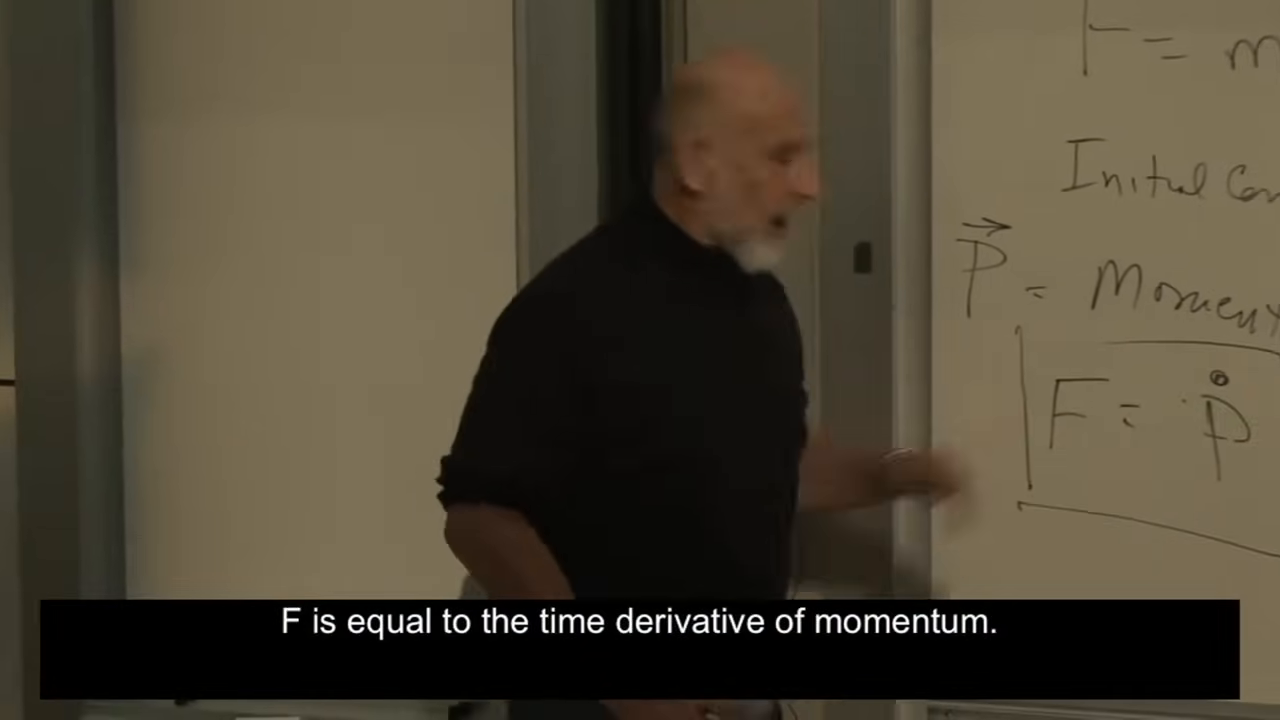
\includegraphics[width=0.82\textwidth]{lecture_02_figure_03.png}\caption{La loi de Newton écrite comme dérivée temporelle de la quantité de mouvement.}\lectureframe{00:32:35}\end{figure}

Pour une coordonnée, le mouvement newtonien peut maintenant s’écrire sous la forme de deux équations du premier ordre portant sur deux variables d’état indépendantes :

\begin{align}
  \dot p&=F(x,t),
  \label{eq:first-order-p}\\
  \dot x&=\frac{p}{m}.
  \label{eq:first-order-x}
\end{align}

L’une des équations indique comment la force modifie la quantité de mouvement ; l’autre, comment la quantité de mouvement modifie la position. Leur forme discrète du premier ordre est

\begin{align}
  p(t+\delta)&=p(t)+\delta F(x(t),t)+O(\delta^2),
  \label{eq:momentum-discrete}\\
  x(t+\delta)&=x(t)+\frac{\delta}{m}p(t)+O(\delta^2).
  \label{eq:position-discrete}
\end{align}

Étant données \(x(t)\) et \(p(t)\), ces équations déterminent la paire suivante, qui sert ensuite de données d’entrée pour l’étape suivante. La trajectoire se construit en répétant ces mises à jour.

\begin{figure}[htbp]\centering
  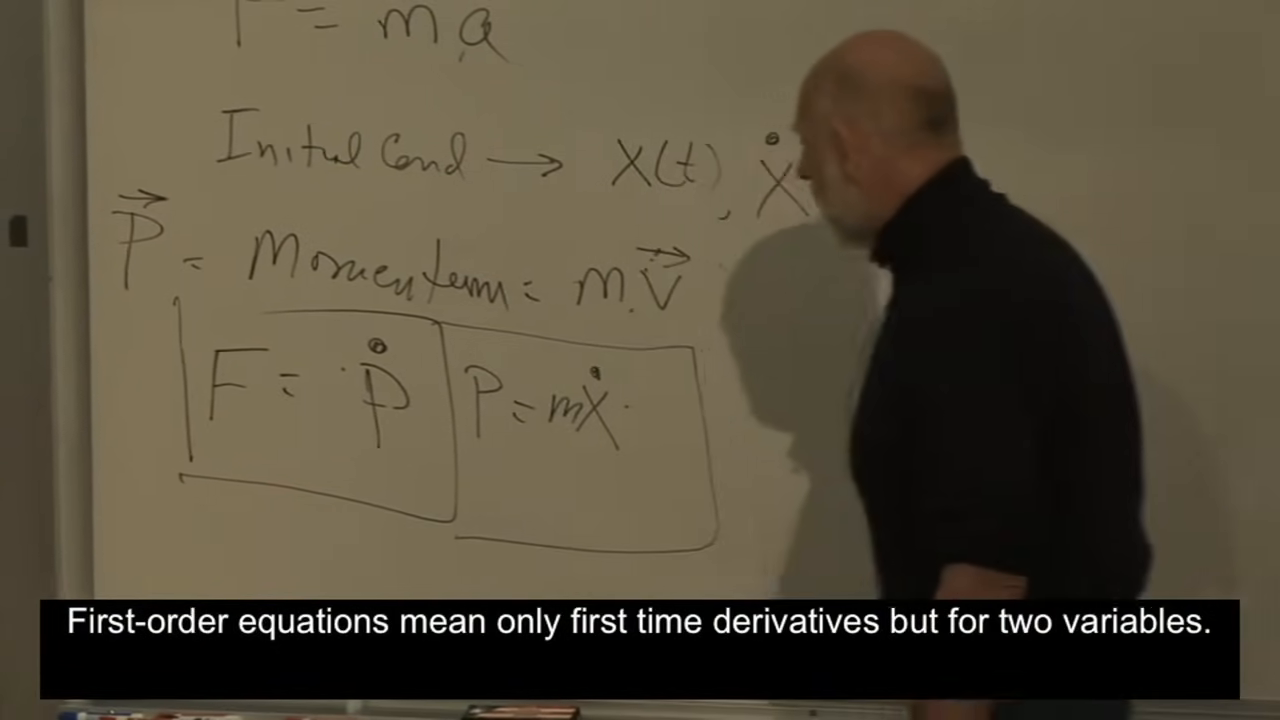
\includegraphics[width=0.84\textwidth]{lecture_02_figure_04.png}\caption{Les deux équations du premier ordre et les données initiales correspondantes. La position et la quantité de mouvement spécifient ensemble l’état.}\lectureframe{00:35:47}\end{figure}

L’ensemble de toutes les paires \((x,p)\) s’appelle l’\emph{espace des phases}. Pour une particule se déplaçant dans trois dimensions, il possède six coordonnées,

\begin{equation}
  (x,y,z,p_x,p_y,p_z).
  \label{eq:one-particle-phase-space}
\end{equation}

L’espace des phases est l’espace des conditions initiales complètes. L’espace des configurations ne décrit que les positions ; l’espace des phases contient précisément les données nécessaires à la loi du mouvement.

\begin{classroomqa}\audiencequestion{Si la force dépend de la position plutôt que du temps selon une fonction connue, la mise à jour devient-elle plus compliquée ?\lecturetimestamp{00:36:27--00:37:07}}\lecturerresponse{Les équations restent prédictives. Une fois que \(x\) et \(p\) sont connus, la valeur de \(F(x)\) est connue. L’équation~\eqref{eq:first-order-p} fait évoluer \(p\), l’équation~\eqref{eq:first-order-x} fait évoluer \(x\), et la paire mise à jour peut être réutilisée.}\end{classroomqa}

\section{Le ressort newtonien}

Revenons au ressort afin de comparer les deux lois dans des conditions physiques identiques. La loi de Newton donne

\begin{equation}
  m\ddot x=-kx.
  \label{eq:newton-spring}
\end{equation}

Posons provisoirement \(m=k=1\) afin d’éliminer les constantes. On obtient alors

\begin{equation}
  \ddot x=-x.
  \label{eq:normalized-oscillator}
\end{equation}

Contrairement à l’exponentielle, un sinus ou un cosinus retrouve son opposé après deux dérivations. La solution générale peut s’écrire

\begin{align}
  x(t)&=C\cos(t-t_0),
  \label{eq:oscillator-x}\\
  p(t)=\dot x(t)&=-C\sin(t-t_0).
  \label{eq:oscillator-p}
\end{align}

Les deux constantes portent les deux informations initiales. L’amplitude \(C\) donne le déplacement maximal, tandis que \(t_0\) fixe la phase, choisie ici de sorte que la vitesse s’annule en \(t=t_0\). La particule s’arrête uniquement de façon momentanée aux extrémités. Elle revient ensuite en passant par l’origine, où sa vitesse et sa quantité de mouvement sont maximales, puis poursuit ses oscillations.

En élevant au carré les équations~\eqref{eq:oscillator-x} et \eqref{eq:oscillator-p}, on obtient

\begin{equation}
  x^2+p^2=C^2.
  \label{eq:oscillator-phase-circle}
\end{equation}

Le point de l’espace des phases se déplace donc sur un cercle de rayon \(C\). Des amplitudes initiales différentes donnent des cercles différents ; modifier \(t_0\) choisit un autre point de départ sur le même cercle. Dans ces unités normalisées, tous les cercles sont parcourus avec la même période \(2\pi\), indépendamment de l’amplitude.

\begin{figure}[htbp]\centering
  \includegraphics[width=0.84\textwidth]{lecture_02_figure_10.png}\caption{Solution de l’oscillateur et orbite circulaire dans le plan de phase \((x,p)\).}\lectureframe{00:43:20}\end{figure}

\begin{figure}[htbp]\centering
  \begin{tikzpicture}[scale=1.05,>=Latex]
    \draw[->] (-2.6,0) -- (2.75,0) node[right] {$x$};
    \draw[->] (0,-2.4) -- (0,2.55) node[above] {$p$};
    \draw[blue!65!black,thick] (0,0) circle (1.85);
    \draw[->,blue!65!black,thick]
      (1.60,0.93) arc[start angle=30,end angle=72,radius=1.85];
    \fill[red!65!black] (1.60,0.93) circle (2pt);
    \draw[dashed] (0,0) -- (1.60,0.93)
      node[midway,below right] {$C$};
    \node[align=left] at (-1.55,1.85)
      {$x=C\cos(t-t_0)$\\$p=-C\sin(t-t_0)$};
  \end{tikzpicture}\caption{Une orbite dans l’espace des phases conserve la position et la quantité de mouvement. Son rayon caractérise le mouvement, tandis que l’angle évolue uniformément au cours du temps.}\label{fig:oscillator-phase-space}\end{figure}

La projection sur l’axe horizontal donne le mouvement de va-et-vient familier de \(x\) ; la projection sur l’axe vertical donne l’oscillation de \(p\). Contrairement au ressort aristotélicien, des cercles distincts ne se confondent jamais. La connaissance d’un point de l’espace des phases détermine à la fois le futur et le passé.

Pour des valeurs générales de \(m\) et \(k\), la pulsation angulaire est

\begin{equation}
  \omega=\sqrt{\frac{k}{m}},
  \qquad
  x(t)=C\cos\bigl(\omega(t-t_0)\bigr),
  \label{eq:general-oscillator-frequency}
\end{equation}

et l’orbite dans l’espace des phases devient une ellipse dans le plan \((x,p)\) non redimensionné. La représentation circulaire correspond à la normalisation commode \(m=k=1\) utilisée dans le cours.

\begin{classroomqa}\audiencequestion{Si, dans l’équation de l’oscillateur, on remplaçait la dérivée seconde par une dérivée première, la prédictibilité serait-elle perdue ?\lecturetimestamp{00:45:23--00:46:04}}\lecturerresponse{Non. Une équation du premier ordre peut quand même prédire le mouvement futur à partir de données initiales appropriées. La question plus profonde est de savoir si son flot préserve suffisamment les distinctions pour être réversible ; nous verrons le théorème général pertinent lorsque nous disposerons des outils nécessaires.}\end{classroomqa}

\section{Renversement du temps}

Le portrait de l’oscillateur rend la réversibilité concrète, mais les équations permettent aussi de la tester directement. Introduisons une coordonnée de temps renversé

\begin{equation}
  T=-t.
  \label{eq:reverse-time}
\end{equation}

On a alors

\begin{equation}
  \frac{d}{dt}=-\frac{d}{dT},
  \qquad
  \frac{d^2}{dt^2}=\frac{d^2}{dT^2}.
  \label{eq:time-derivative-parity}
\end{equation}

Une dérivée première change de signe sous le renversement du temps, contrairement à une dérivée seconde. Par conséquent, l’équation aristotélicienne autonome

\begin{equation}
  m\dot x=F(x)
  \label{eq:aristotle-time-reversal}
\end{equation}

ne conserve pas sa forme lorsqu’on passe le film à l’envers. Un ressort qui se rapproche de l’équilibre se mettrait à s’en éloigner spontanément. En revanche,

\begin{equation}
  m\ddot x=F(x)
  \label{eq:newton-time-reversal}
\end{equation}

reste inchangée. Lorsqu’on inverse un film newtonien, la vitesse s’inverse, mais l’accélération demeure inchangée ; le film inversé est donc une autre solution admissible.

\begin{figure}[htbp]\centering
  \includegraphics[width=0.84\textwidth]{lecture_02_figure_11.png}\caption{Comparaison au tableau sous la transformation \(t\mapsto -t\) : les dérivées premières changent de signe, contrairement aux dérivées secondes.}\lectureframe{00:50:45}\end{figure}

\begin{classroomqa}\audiencequestion{Pourquoi accepter la réversibilité comme principe général en physique ?\lecturetimestamp{00:46:16--00:48:26}}\lecturerresponse{On la met à l’épreuve ; elle n’est pas garantie par définition. Nous examinons les lois qui ont fait leurs preuves, repérons les caractéristiques communes aux expériences et érigeons celles-ci en principes. L’ordre logique plus profond est inverse : la théorie quantique des champs est plus fondamentale, et la mécanique newtonienne en émerge par des approximations telles que le mouvement lent et les objets massifs. Un cours doit progresser à partir de lois plus simples ; la réversibilité est donc introduite ici comme un principe dont la portée sera mise à l’épreuve par la suite.}\end{classroomqa}

\begin{classroomqa}\audiencequestion{Newton avait-il lui-même reconnu consciemment la réversibilité comme un problème ?\lecturetimestamp{00:48:28--00:49:02}}\lecturerresponse{La réponse historique est incertaine. Newton comprenait certainement l’inertie : une force est nécessaire pour modifier un état de mouvement, pas pour entretenir un mouvement uniforme. La question de savoir s’il a formulé explicitement cette idée en termes de réversibilité est une question historique distincte.}\end{classroomqa}

\section{Cycles et grandeurs conservées}

Les cercles de l’espace des phases suggèrent l’idée suivante. Une trajectoire reste sur un cercle donné et ne saute jamais sur un autre. On peut donc associer au cercle un nombre qui reste constant au cours du mouvement. Pour l’oscillateur normalisé, ce nombre est

\begin{equation}
  C^2=x^2+p^2.
  \label{eq:cycle-label}
\end{equation}

À un facteur deux près, il s’agit de l’énergie de l’oscillateur. Les cercles de plus grand rayon correspondent à une énergie plus élevée ; changer la phase initiale ne la modifie pas. Nous allons dériver ce résultat plutôt que de simplement le lire sur le schéma, mais considérons d’abord la quantité de mouvement.

La première loi de Newton affirme qu’un objet soumis à une force nette nulle se déplace à vitesse constante. Ce résultat est déjà contenu dans la deuxième loi :

\begin{equation}
  \mathbf F=0
  \quad\Longrightarrow\quad
  \dot{\mathbf p}=0
  \quad\Longrightarrow\quad
  \mathbf v=\text{constant}
  \label{eq:newton-first-from-second}
\end{equation}

lorsque la masse est constante. La troisième loi de Newton apporte une information véritablement nouvelle sur les interactions entre particules.

\subsection{Forces égales, opposées et centrales}

Notons \(\mathbf F_{ij}\) la force exercée sur la particule \(i\) par la particule \(j\). La relation d’égalité et d’opposition de la troisième loi s’écrit

\begin{equation}
  \mathbf F_{ij}=-\mathbf F_{ji}.
  \label{eq:newton-third-pair}
\end{equation}

Si les deux forces pointaient dans la même direction, une paire isolée pourrait accélérer spontanément. Elle constituerait une machine sans propulseur, produisant du mouvement par les seules forces internes. On n’observe pas un tel comportement.

\begin{figure}[htbp]\centering
  \includegraphics[width=0.84\textwidth]{lecture_02_figure_12.png}\caption{Énoncé indicé des forces d’interaction égales et opposées.}\lectureframe{00:59:25}\end{figure}

Pour les forces entre particules ponctuelles considérées ici, les forces de la paire agissent aussi le long de la droite qui joint les centres des particules. Des forces égales et opposées mais non colinéaires pourraient former un couple pur et mettre en rotation une paire rigide isolée. La condition de centralité empêche cette possibilité :

\begin{equation}
  \mathbf F_{ij}\parallel
  (\mathbf r_i-\mathbf r_j).
  \label{eq:central-force-condition}
\end{equation}

La condition d’égalité et d’opposition entraînera la conservation de la quantité de mouvement linéaire. La condition relative à la droite des centres est liée à la conservation du moment cinétique, qui sera étudiée plus tard.

\begin{figure}[htbp]\centering
  \includegraphics[width=0.84\textwidth]{lecture_02_figure_13.png}\caption{La condition de centralité dans la troisième loi de Newton : les forces d’interaction sont dirigées le long de la droite qui joint les particules.}\lectureframe{01:01:38}\end{figure}

\subsection{Quantité de mouvement totale}

Considérons un système fermé de \(N\) particules. Il n’y a aucune force extérieure ; les seules forces sont celles que les particules exercent les unes sur les autres. L’additivité des forces et la deuxième loi de Newton donnent, pour chaque particule,

\begin{equation}
  \dot{\mathbf p}_i
  =m_i\ddot{\mathbf r}_i
  =\sum_{\substack{j=1\\j\ne i}}^N \mathbf F_{ij}.
  \label{eq:many-particle-newton}
\end{equation}

Faisons la somme de cette équation sur \(i\) :

\begin{align}
  \frac{d}{dt}\sum_{i=1}^N\mathbf p_i
  &=\sum_{i=1}^N
    \sum_{\substack{j=1\\j\ne i}}^N\mathbf F_{ij}
  \notag\\
  &=\sum_{i<j}\bigl(\mathbf F_{ij}+\mathbf F_{ji}\bigr)
  =0.
  \label{eq:momentum-pair-cancellation}
\end{align}

Chaque interaction apparaît deux fois, une fois dans chaque sens, et les forces de la paire s’annulent. En définissant

\begin{equation}
  \mathbf P_{\mathrm{tot}}=\sum_{i=1}^N\mathbf p_i,
  \label{eq:total-momentum}
\end{equation}

on obtient la première loi de conservation :

\begin{equation}
  \frac{d\mathbf P_{\mathrm{tot}}}{dt}=0.
  \label{eq:momentum-conservation}
\end{equation}

\begin{figure}[htbp]\centering
  \includegraphics[width=0.84\textwidth]{lecture_02_figure_14.png}\caption{En sommant les équations des particules, les forces deux à deux s’annulent ; il ne reste que la dérivée de la quantité de mouvement totale, égale à zéro.}\lectureframe{01:04:38}\end{figure}

Historiquement, nous avons présenté la conservation de la quantité de mouvement comme une conséquence de la troisième loi de Newton. La physique moderne considère souvent cette conservation comme l’énoncé le plus fondamental : si un système isolé à deux particules conserve sa quantité de mouvement totale, les variations de leurs quantités de mouvement internes doivent être égales et opposées. Pour le développement présent, toutefois, la démarche newtonienne est la plus utile.

\section{Énergie en une dimension}

Considérons une particule se déplaçant sur une droite sous l’action d’une force qui dépend uniquement de sa position :

\begin{equation}
  F=F(x).
  \label{eq:position-force}
\end{equation}

Une telle force est dite indépendante du temps. Cela ne signifie pas que la valeur numérique de la force subie par la particule en mouvement soit constante. Sa valeur change lorsque \(x(t)\) change. Cela signifie que, chaque fois que la particule se trouve à la même position \(x\), elle subit la même force, quelle que soit l’heure indiquée par l’horloge.

En une dimension, toute fonction de force suffisamment régulière peut être intégrée. Nous définissons donc une énergie potentielle \(V(x)\) par

\begin{equation}
  F(x)=-\frac{dV}{dx},
  \label{eq:potential-definition-1d}
\end{equation}

ou, de manière équivalente,

\begin{equation}
  V(x)=-\int^x F(u)\,du+V_0.
  \label{eq:potential-integral}
\end{equation}

La constante additive \(V_0\) n’a aucun effet sur la force. Représentons \(V(x)\) comme la hauteur d’un paysage au-dessus de l’axe \(x\). La particule est poussée vers les hauteurs plus faibles, et la force est d’autant plus grande que la pente est raide. Au sommet ou au creux d’une colline lisse, la pente s’annule, et la force aussi.

\begin{figure}[htbp]\centering
  \includegraphics[width=0.84\textwidth]{lecture_02_figure_15.png}\caption{L’énergie potentielle comme paysage unidimensionnel. La force est dirigée vers le bas de la pente et son intensité est déterminée par la pente.}\lectureframe{01:12:57}\end{figure}

Définissons les énergies cinétique, potentielle et totale par

\begin{equation}
  T=\frac12m\dot x^2,
  \qquad
  E=T+V(x)
  =\frac12m\dot x^2+V(x).
  \label{eq:energy-1d}
\end{equation}

À ce stade, énergie est simplement le nom donné à cette quantité candidate à la conservation. Le paysage suggère son interprétation physique : en descendant la pente, \(V\) diminue tandis que la vitesse augmente, et donc \(T\) aussi ; en remontant la pente, c’est l’inverse. L’équation de Newton démontre que cet échange est exact.

Dérivons l’équation~\eqref{eq:energy-1d}. Puisque \(m\) est constante et que \(V\) ne dépend du temps qu’à travers \(x(t)\),

\begin{align}
  \frac{dE}{dt}
  &=m\dot x\ddot x+\frac{dV}{dx}\dot x
  \notag\\
  &=\dot x\left(m\ddot x+\frac{dV}{dx}\right).
  \label{eq:energy-derivative-1d}
\end{align}

La loi de Newton et la définition de \(V\) donnent

\begin{equation}
  m\ddot x=F=-\frac{dV}{dx}.
  \label{eq:newton-potential-1d}
\end{equation}

Le terme entre crochets dans l’équation~\eqref{eq:energy-derivative-1d} s’annule donc :

\begin{equation}
  \frac{dE}{dt}=0.
  \label{eq:energy-conservation-1d}
\end{equation}

\begin{figure}[htbp]\centering
  \includegraphics[width=0.84\textwidth]{lecture_02_figure_16.png}\caption{La dérivée de l’énergie unidimensionnelle, factorisée en un produit de la vitesse par l’équation de Newton.}\lectureframe{01:19:18}\end{figure}

En une dimension, aucune hypothèse dynamique supplémentaire n’était nécessaire au-delà d’une force régulière dépendant de la position, car toute force de ce type possède une primitive.

\section{Plusieurs dimensions et forces conservatives}

Pour une particule de coordonnées \(x_i\), l’équation de Newton se décompose en

\begin{equation}
  F_i(\mathbf x)=m\ddot x_i.
  \label{eq:newton-components}
\end{equation}

La composante \(F_i\) de la force peut dépendre de toutes les coordonnées, et pas seulement de \(x_i\). Nous aimerions trouver une fonction scalaire unique \(V(\mathbf x)\) telle que

\begin{equation}
  F_i(\mathbf x)
  =-\frac{\partial V(\mathbf x)}{\partial x_i},
  \qquad
  \mathbf F=-\boldsymbol\nabla V.
  \label{eq:gradient-force}
\end{equation}

Contrairement à la construction unidimensionnelle, cela n’est pas automatique. Trois fonctions arbitraires \(F_1,F_2,F_3\) contiennent en général davantage d’informations indépendantes que les dérivées d’une seule fonction scalaire. De manière équivalente, un potentiel n’existe que si le champ de forces satisfait des conditions de compatibilité, telles que l’égalité des dérivées partielles mixtes appropriées ; dans une région simplement connexe, cela s’exprime par \(\boldsymbol\nabla\times\mathbf F=0\). Nous posons donc l’équation~\eqref{eq:gradient-force} comme un postulat physique pour la classe de forces considérée, et non comme une identité mathématique.

\begin{figure}[htbp]\centering
  \includegraphics[width=0.84\textwidth]{lecture_02_figure_17.png}\caption{La loi des forces en plusieurs dimensions et un schéma des courbes de niveau du potentiel. La force pointe à travers les courbes de niveau, vers les valeurs décroissantes de \(V\).}\lectureframe{01:24:15}\end{figure}

Sur une carte de contours, \(V\) est constant le long de chaque courbe de niveau. Le gradient est perpendiculaire à ces courbes et pointe dans la direction de la plus forte augmentation ; la force \(-\boldsymbol\nabla V\) pointe dans la direction de la plus forte diminution.

\begin{figure}[htbp]\centering
  \begin{tikzpicture}[scale=1.0,>=Latex]
    \draw[->] (-3.0,0) -- (3.1,0) node[right] {$x_1$};
    \draw[->] (0,-2.4) -- (0,2.55) node[above] {$x_2$};
    \draw[orange!65!black,thick]
      plot[smooth cycle] coordinates
      {(-0.55,-0.35) (0.15,-0.55) (0.72,-0.10) (0.50,0.53) (-0.25,0.65)};
    \draw[orange!65!black,thick]
      plot[smooth cycle] coordinates
      {(-1.15,-0.75) (0.20,-1.10) (1.35,-0.25) (1.10,0.95) (-0.45,1.25)};
    \draw[orange!65!black,thick]
      plot[smooth cycle] coordinates
      {(-1.85,-1.20) (0.15,-1.70) (2.15,-0.40) (1.70,1.50) (-0.80,1.85)};
    \draw[->,blue!65!black,very thick] (1.62,0.73) -- (0.82,0.20)
      node[midway,above left] {$\mathbf F$};
    \draw[dashed,->,red!65!black,thick] (0.82,0.20) -- (1.62,0.73)
      node[midway,below right] {$\boldsymbol\nabla V$};
    \node[orange!65!black] at (-1.62,1.45) {$V=V_3$};
    \node[orange!65!black] at (-0.92,0.92) {$V=V_2$};
    \node[orange!65!black] at (-0.35,0.30) {$V=V_1$};
  \end{tikzpicture}\caption{Courbes de niveau d’un potentiel scalaire. Le gradient est normal aux courbes de niveau, et une force conservative pointe dans la direction opposée.}\label{fig:potential-contours}\end{figure}

Lorsque l’équation~\eqref{eq:gradient-force} est vérifiée, définissons

\begin{equation}
  E=\frac12m\sum_i\dot x_i^2+V(x_1,\ldots,x_n).
  \label{eq:energy-many-coordinates}
\end{equation}

Le terme cinétique est égal à la moitié du produit de la masse par le carré de la norme du vecteur vitesse. En dérivant et en appliquant la règle de dérivation en chaîne pour plusieurs variables, on obtient

\begin{align}
  \frac{dE}{dt}
  &=m\sum_i\dot x_i\ddot x_i
    +\sum_i\frac{\partial V}{\partial x_i}\dot x_i
  \notag\\
  &=\sum_i\dot x_i
    \left(m\ddot x_i+\frac{\partial V}{\partial x_i}\right)
  =0.
  \label{eq:energy-derivative-multidimensional}
\end{align}

La démonstration est exactement celle du cas unidimensionnel, avec un indice en plus, mais son hypothèse est plus forte : toutes les composantes de la force doivent dériver d’un même potentiel.

\begin{figure}[htbp]\centering
  \includegraphics[width=0.84\textwidth]{lecture_02_figure_18.png}\caption{Dérivée indicée de l’énergie. Chaque terme entre crochets s’annule grâce à la composante correspondante de l’équation de Newton.}\lectureframe{01:28:30}\end{figure}

Pour \(N\) particules en trois dimensions, rassemblons toutes les coordonnées dans une seule liste

\begin{equation}
  \begin{aligned}
    q_a={}&(x_1,y_1,z_1,x_2,y_2,z_2,\ldots,\\[-0.2em]
           &\phantom{(}x_N,y_N,z_N),\\
    &a=1,\ldots,3N.
  \end{aligned}
  \label{eq:flattened-coordinates}
\end{equation}

Il y a \(3N\) coordonnées, mais seulement \(N\) masses ; une même masse intervient dans les trois coordonnées associées à une particule donnée. Si

\begin{equation}
  F_a=-\frac{\partial V(q_1,\ldots,q_{3N})}{\partial q_a},
  \label{eq:many-particle-conservative-force}
\end{equation}

alors

\begin{equation}
  E=\sum_{A=1}^{N}\frac12m_A\lvert\dot{\mathbf r}_A\rvert^2
    +V(\mathbf r_1,\ldots,\mathbf r_N)
  \label{eq:many-particle-energy}
\end{equation}

est conservée par le même calcul. Les forces qui dérivent d’un potentiel sont dites \emph{conservatives} précisément parce qu’elles permettent cette loi de conservation ; l’adjectif n’a aucun sens politique.

\section{L’oscillateur comme courbe de niveau d’énergie}\enlargethispage{3\baselineskip}

Pour la force de rappel du ressort \(F=-kx\), l’équation~\eqref{eq:potential-definition-1d} donne

\begin{equation}
  V(x)=\frac12kx^2+V_0.
  \label{eq:spring-potential}
\end{equation}

En choisissant \(V_0=0\), l’énergie de l’oscillateur est

\begin{equation}
  E=\frac12m\dot x^2+\frac12kx^2
   =\frac{p^2}{2m}+\frac12kx^2.
  \label{eq:oscillator-energy}
\end{equation}

Pour \(m=k=1\),

\begin{equation}
  2E=p^2+x^2=C^2.
  \label{eq:oscillator-energy-circle}
\end{equation}

Les cercles de l’espace des phases obtenus précédemment sont donc des courbes de niveau d’énergie constante. Pour un potentiel unidimensionnel plus général, ces courbes ne sont pas nécessairement circulaires, mais le mouvement reste situé sur des courbes

\begin{equation}
  \frac{p^2}{2m}+V(x)=E
  \label{eq:general-energy-contour}
\end{equation}

dans le plan \((x,p)\). Nous retrouvons ainsi l’idée de la première leçon : lorsque les trajectoires restent sur des cycles ou des orbites distincts, un nombre peut caractériser ces orbites et rester inchangé tout au long du mouvement.

Nous disposons maintenant de l’espace des états, des équations de mise à jour newtoniennes et des deux premières lois de conservation. La prochaine formulation de la mécanique partira du principe de moindre action et conduira aux lagrangiens, aux hamiltoniens, au moment cinétique et à la structure plus générale qui sous-tend ces exemples.

\begin{classroomqa}\audiencequestion{Dans quelle mesure le polycopié distribué correspond-il au travail effectué au tableau, et où sont les figures ?\lecturetimestamp{01:37:56--01:38:54}}\lecturerresponse{Le polycopié devrait suivre de près le cours ; si certains éléments présentés au tableau n’y figurent pas, il se peut que le mauvais fichier ait été envoyé. Les figures n’étaient pas encore prêtes ; comme il le plaisante, elles arriveraient quand la formation continue paierait le prochain chèque.}\end{classroomqa}